After the global matrices assembly, the boundary conditions are applied. 
As was said in the section \ref{trimesh}, during the mesh import 
it is possible to identify the nodes that they are in the boundary. 
The condition where the nodes have their values predefined 
by the problem is known as \textit{Dirichlet condition}. 
Therefore, these nodes must not be changed as the simulation is 
performed. In this way, the product between the column of the 
global matrix whose index is a node with Dirichlet boundary condition 
and its predefined value as boundary condition is subtracted from 
the vector on the right side of the governing equation. 
Then, we zero the rows and columns of the global matrix that 
corresponds to the condition index of Dirichlet and we set the value 
of 1 on the main diagonal.

\medskip
Para exemplificar, consideraremos uma matriz 
com dimensões (\textit{np x np})
e o nó 2 como um nó localizado no
contorno do domínio onde a condição proposta
é de Dirichlet.
Desta forma, o seguinte algoritmo é feito conforme apresentado por Anjos (2007) \cite{anjos2007}:

\begin{enumerate}
 
 \vspace{0.5cm}
 \item \textbf{Localiza-se o nó de condição de contorno na matriz:}
\medskip
\begin{center}
\begin{tikzpicture}
\matrix (m) [matrix of math nodes,
inner sep=0pt, column sep=0.4em,
nodes={inner sep=0.4em,text width=1.0em,align=center},
left delimiter={[},
right delimiter={]},
]
{
a_{11} & a_{12} & a_{13} & \cdots & a_{1j} & \cdots & a_{1n} \\
a_{21} & a_{22} & a_{23} & \cdots & a_{2j} & \cdots & a_{2n} \\
a_{31} & a_{32} & a_{33} & \cdots & a_{3j} & \cdots & a_{3n} \\
\vdots & \vdots & \vdots & \ddots & \vdots & \vdots & \vdots \\
a_{n1} & a_{n2} & a_{n3} & \cdots & a_{nj} & \cdots & a_{nn} \\
};
\begin{scope}[xshift=4.2cm]
\matrix (m) [matrix of math nodes,
inner sep=0pt, column sep=0.4em,
nodes={inner sep=0.4em,text width=1em,align=center},
left delimiter={[},
right delimiter={]},
]
{
c_1 \\
c_2 \\
c_3 \\
\vdots \\
c_n \\
};
\end{scope}
\begin{scope}[xshift=5.2cm]
\node {=};
\end{scope}
\begin{scope}[xshift=6.2cm]
\matrix (m) [matrix of math nodes,
inner sep=0pt, column sep=0.4em,
nodes={inner sep=0.3em,text width=0.8em,align=center},
left delimiter={[},
right delimiter={]},
]
{
b_1 \\
b_2 \\
b_3 \\
\vdots \\
b_n \\
};
\end{scope}
 \draw[<-] (-1.5,-1.8) -- (-1.5,-2.5) -- (-1.1,-2.5);
 \node [draw=none, align=right] at (2.0,-2.5) {Identificar a coluna cujo índice é \\ condição de contorno de Dirichlet};
\end{tikzpicture}
\end{center}

 \vspace{0.5cm}
 \item \textbf{Subtrai-se o produto entre a coluna onde está situado o nó da matriz e o seu valor pré definido 
com o vetor do lado direito da equação:}
\medskip
\begin{center}
\begin{tikzpicture}
\matrix (m) [matrix of math nodes,
inner sep=0pt, column sep=0.4em,
nodes={inner sep=0.4em,text width=1.0em,align=center},
left delimiter={[},
right delimiter={]},
]
{
a_{11} & a_{12} & a_{13} & \cdots & a_{1j} & \cdots & a_{1n} \\
a_{21} & a_{22} & a_{23} & \cdots & a_{2j} & \cdots & a_{2n} \\
a_{31} & a_{32} & a_{33} & \cdots & a_{3j} & \cdots & a_{3n} \\
\vdots & \vdots & \vdots & \ddots & \vdots & \vdots & \vdots \\
a_{n1} & a_{n2} & a_{n3} & \cdots & a_{nj} & \cdots & a_{nn} \\
};
\begin{scope}[xshift=4.2cm]
\matrix (m) [matrix of math nodes,
inner sep=0pt, column sep=0.4em,
nodes={inner sep=0.4em,text width=1em,align=center},
left delimiter={[},
right delimiter={]},
]
{
c_1 \\
c_2 \\
c_3 \\
\vdots \\
c_n \\
};
\end{scope}
\begin{scope}[xshift=5.2cm]
\node {=};
\end{scope}
\begin{scope}[xshift=6.2cm]
\matrix (m) [matrix of math nodes,
inner sep=0pt, column sep=0.4em,
nodes={inner sep=0.3em,text width=0.8em,align=center},
left delimiter={[},
right delimiter={]},
]
{
b_1 \\
b_2 \\
b_3 \\
\vdots \\
b_n \\
};
\end{scope}
 %text
 \draw[<-] (-1.5,-1.8) -- (-1.5,-2.5) -- (-1.1,-2.5);
 \node [draw=none, align=right] at (2.5,-2.5) {Subtrair o produto desta coluna com o \\ valor de $c_2$ no lado direito da equação};
 %block
 \draw[red] (-1.9,1.8) -- (-1.15,1.8) -- (-1.15,-1.7) -- (-1.9,-1.7) -- cycle;
 \draw[red] (3.9,0.95) -- (4.5,0.95) -- (4.5,0.45) -- (3.9,0.45) -- cycle;
\end{tikzpicture}
\end{center}

\newpage
isto é,

\medskip
\begin{center}
\begin{tikzpicture}
\matrix (m) [matrix of math nodes,
inner sep=0pt, column sep=0.4em,
nodes={inner sep=0.4em,text width=1.0em,align=center},
left delimiter={[},
right delimiter={]},
]
{
a_{11} & a_{12} & a_{13} & \cdots & a_{1j} & \cdots & a_{1n} \\
a_{21} & a_{22} & a_{23} & \cdots & a_{2j} & \cdots & a_{2n} \\
a_{31} & a_{32} & a_{33} & \cdots & a_{3j} & \cdots & a_{3n} \\
\vdots & \vdots & \vdots & \ddots & \vdots & \vdots & \vdots \\
a_{n1} & a_{n2} & a_{n3} & \cdots & a_{nj} & \cdots & a_{nn} \\
};
\begin{scope}[xshift=4.2cm]
\matrix (m) [matrix of math nodes,
inner sep=0pt, column sep=0.4em,
nodes={inner sep=0.4em,text width=1em,align=center},
left delimiter={[},
right delimiter={]},
]
{
c_1 \\
c_2 \\
c_3 \\
\vdots \\
c_n \\
};
\end{scope}
\begin{scope}[xshift=5.2cm]
\node {=};
\end{scope}
\begin{scope}[xshift=6.2cm]
\matrix (m) [matrix of math nodes,
inner sep=0pt, column sep=0.4em,
nodes={inner sep=0.3em,text width=0.8em,align=center},
left delimiter={[},
right delimiter={]},
]
{
b_1 \\
b_2 \\
b_3 \\
\vdots \\
b_n \\
};
\end{scope}
\begin{scope}[xshift=7.2cm]
\node {-};
\end{scope}
\begin{scope}[xshift=8.2cm]
\matrix (m) [matrix of math nodes,
inner sep=0pt, column sep=0.4em,
nodes={inner sep=0.4em,text width=1em,align=center},
left delimiter={[},
right delimiter={]},
]
{
a_{12} \\
a_{22} \\
a_{32} \\
\vdots \\
a_{n2} \\
};
\end{scope}
\begin{scope}[xshift=9.0cm]
\node {*};
\end{scope}
\begin{scope}[xshift=9.4cm]
 \node {$c_2$};
\end{scope}
 %text
 \node [draw=none, align=right] at (8.5,-2.6) {$bc\_dirichlet$};
 %block
 \draw (7.3,-1.7) -- (7.3,-2.0) -- (9.7,-2.0) -- (9.7,-1.7);
 \draw (8.5,-2.0) -- (8.5,-2.3);
\end{tikzpicture}
\end{center}

 \vspace{0.5cm}
 \item \textbf{Preenche-se com zeros a coluna e a linha da matriz correspondente ao nó de condição de contorno:}
\medskip
\begin{center}
\begin{tikzpicture}
\matrix (m) [matrix of math nodes,
inner sep=0pt, column sep=0.4em,
nodes={inner sep=0.4em,text width=1.0em,align=center},
left delimiter={[},
right delimiter={]},
]
{
a_{11} & 0 & a_{13} & \cdots & a_{1j} & \cdots & a_{1n} \\
0 & 0 & 0 & \cdots & 0 & \cdots & 0 \\
a_{31} & 0 & a_{33} & \cdots & a_{3j} & \cdots & a_{3n} \\
\vdots & \vdots & \vdots & \ddots & \vdots & \vdots & \vdots \\
a_{n1} & 0 & a_{n3} & \cdots & a_{nj} & \cdots & a_{nn} \\
};
\begin{scope}[xshift=4.2cm]
\matrix (m) [matrix of math nodes,
inner sep=0pt, column sep=0.4em,
nodes={inner sep=0.4em,text width=1em,align=center},
left delimiter={[},
right delimiter={]},
]
{
c_1 \\
c_2 \\
c_3 \\
\vdots \\
c_n \\
};
\end{scope}
\begin{scope}[xshift=5.2cm]
\node {=};
\end{scope}
\begin{scope}[xshift=6.2cm]
\matrix (m) [matrix of math nodes,
inner sep=0pt, column sep=0.4em,
nodes={inner sep=0.3em,text width=0.8em,align=center},
left delimiter={[},
right delimiter={]},
]
{
b_1 \\
b_2 \\
b_3 \\
\vdots \\
b_n \\
};
\end{scope}
\begin{scope}[xshift=7.2cm]
\node {-};
\end{scope}
\begin{scope}[xshift=8.2cm]
\matrix (m) [matrix of math nodes,
inner sep=0pt, column sep=0.4em,
nodes={inner sep=0.4em,text width=1em,align=center},
left delimiter={[},
right delimiter={]},
]
{
a_{12} \\
a_{22} \\
a_{32} \\
\vdots \\
a_{n2} \\
};
\end{scope}
\begin{scope}[xshift=9.0cm]
\node {*};
\end{scope}
\begin{scope}[xshift=9.4cm]
 \node {$c_2$};
\end{scope}
\end{tikzpicture}
\end{center}


 \vspace{0.5cm}
 \item \textbf{Coloca-se 1 na diagonal principal da matriz cujo índice é o nó de condição de contorno:}
\medskip
\begin{center}
\begin{tikzpicture}
\matrix (m) [matrix of math nodes,
inner sep=0pt, column sep=0.4em,
nodes={inner sep=0.4em,text width=1.0em,align=center},
left delimiter={[},
right delimiter={]},
]
{
a_{11} & 0 & a_{13} & \cdots & a_{1j} & \cdots & a_{1n} \\
0 & 1 & 0 & \cdots & 0 & \cdots & 0 \\
a_{31} & 0 & a_{33} & \cdots & a_{3j} & \cdots & a_{3n} \\
\vdots & \vdots & \vdots & \ddots & \vdots & \vdots & \vdots \\
a_{n1} & 0 & a_{n3} & \cdots & a_{nj} & \cdots & a_{nn} \\
};
\begin{scope}[xshift=4.2cm]
\matrix (m) [matrix of math nodes,
inner sep=0pt, column sep=0.4em,
nodes={inner sep=0.4em,text width=1em,align=center},
left delimiter={[},
right delimiter={]},
]
{
c_1 \\
c_2 \\
c_3 \\
\vdots \\
c_n \\
};
\end{scope}
\begin{scope}[xshift=5.2cm]
\node {=};
\end{scope}
\begin{scope}[xshift=6.2cm]
\matrix (m) [matrix of math nodes,
inner sep=0pt, column sep=0.4em,
nodes={inner sep=0.3em,text width=0.8em,align=center},
left delimiter={[},
right delimiter={]},
]
{
b_1 \\
b_2 \\
b_3 \\
\vdots \\
b_n \\
};
\end{scope}
\begin{scope}[xshift=7.2cm]
\node {-};
\end{scope}
\begin{scope}[xshift=8.2cm]
\matrix (m) [matrix of math nodes,
inner sep=0pt, column sep=0.4em,
nodes={inner sep=0.4em,text width=1em,align=center},
left delimiter={[},
right delimiter={]},
]
{
a_{12} \\
a_{22} \\
a_{32} \\
\vdots \\
a_{n2} \\
};
\end{scope}
\begin{scope}[xshift=9.0cm]
\node {*};
\end{scope}
\begin{scope}[xshift=9.4cm]
 \node {$c_2$};
\end{scope}
\end{tikzpicture}
\end{center}

 \vspace{0.5cm}
 \item \textbf{Localiza-se o próximo nó e executa-se o passo novamente.}
\end{enumerate}

\newpage
\noindent
A implementação deste algoritmo foi realizado pelo seguinte \textit{script}:
\begin{verbatim}
__________________________________________________________________________
 for mm in ibc:                        | loop sobre os nós do contorno
  bc_dirichlet -= LHS[:,mm]*bc_1[mm]   | passo 2
  LHS[:,mm] = 0.0                      | passo 3 - zerar colunas
  LHS[mm,:] = 0.0                      | passo 3 - zerar linhas
  LHS[mm,mm] = 1.0                     | passo 4 - 1 na diagonal principal
  bc_dirichlet[mm] = bc_1[mm]          | imputando o valor da condição
                                       | de Dirichlet no índice
                                       | correspondente
__________________________________________________________________________
\end{verbatim}

\noindent
onde \textit{ibc} é uma lista que contém todos os nós do contorno
cuja condição é de Dirichlet e
\textit{$bc\_1$} é um vetor auxiliar com dimensão \textit{np}
onde o valor da condição de Dirichlet é imputada em cada índice correspondente.
O símbolo -= garante que a contribuição de cada nó cuja
condição seja de Dirichlet seja computada.
Este procedimento deverá ser realizado para cada um das \textit{LHS}.
A \ref{tempo contorno} apresenta o tempo de processamento para 
a aplicação das condições de contorno de \textit{Dirichlet} em diversas
malhas triangulares lineares não estruturadas.

\vspace{0.5cm}
\begin{table}[H]
\centering
\begin{tabular}{ccc}
\toprule
\textbf{N. Nós} & \textbf{N. Elementos} & \textbf{Tempo de Processamento} (s) \\
\midrule
10482 & 20142 & 6,8 \\
40819 & 80005 & 37,5 \\
249677 & 495289 & 467,7 \\
993091 & 2010501 & 3720,6 \\
\bottomrule
\end{tabular}
\caption{Tempo processamento para as condições de contorno para diversas malhas triangulares não estruturadas}
\label{tempo contorno}
\end{table}
 

\medskip
Outro tipo de condição de contorno muito comum é aquela onde existe um
fluxo nos contornos do domínio. Essa condição de contorno é conhecida
como \textit{Condição de Neumann} e na formulação variacional é chamada
de \textit{Condição Natural}. Diferente da condição de Dirichlet,
esse tipo de condição de contorno não afeta a matriz global do lado esquerdo quando
o fluxo é constante. Devemos apenas somar a sua contribuição
no vetor do lado direito da equação, isto é:

\begin{center}
\begin{tikzpicture}
\matrix (m) [matrix of math nodes,
inner sep=0pt, column sep=0.4em,
nodes={inner sep=0.4em,text width=1.0em,align=center},
left delimiter={[},
right delimiter={]},
]
{
a_{11} & 0 & a_{13} & \cdots & a_{1j} & \cdots & a_{1n} \\
0 & 1 & 0 & \cdots & 0 & \cdots & 0 \\
a_{31} & 0 & a_{33} & \cdots & a_{3j} & \cdots & a_{3n} \\
\vdots & \vdots & \vdots & \ddots & \vdots & \vdots & \vdots \\
a_{n1} & 0 & a_{n3} & \cdots & a_{nj} & \cdots & a_{nn} \\
};
\begin{scope}[xshift=4.2cm]
\matrix (m) [matrix of math nodes,
inner sep=0pt, column sep=0.4em,
nodes={inner sep=0.4em,text width=1em,align=center},
left delimiter={[},
right delimiter={]},
]
{
c_1 \\
c_2 \\
c_3 \\
\vdots \\
c_n \\
};
\end{scope}
\begin{scope}[xshift=5.2cm]
\node {=};
\end{scope}
\begin{scope}[xshift=6.2cm]
\matrix (m) [matrix of math nodes,
inner sep=0pt, column sep=0.4em,
nodes={inner sep=0.3em,text width=0.8em,align=center},
left delimiter={[},
right delimiter={]},
]
{
b_1 \\
b_2 \\
b_3 \\
\vdots \\
b_n \\
};
\end{scope}
\begin{scope}[xshift=7.2cm]
\node {-};
\end{scope}
\begin{scope}[xshift=8.2cm]
\matrix (m) [matrix of math nodes,
inner sep=0pt, column sep=0.4em,
nodes={inner sep=0.4em,text width=1em,align=center},
left delimiter={[},
right delimiter={]},
]
{
a_{12} \\
a_{22} \\
a_{32} \\
\vdots \\
a_{n2} \\
};
\end{scope}
\begin{scope}[xshift=9.0cm]
\node {*};
\end{scope}
\begin{scope}[xshift=9.4cm]
 \node {$c_2$};
\end{scope}
\begin{scope}[xshift=10.0cm]
\node {+};
\end{scope}
\begin{scope}[xshift=11.0cm]
\matrix (m) [matrix of math nodes,
inner sep=0pt, column sep=0.4em,
nodes={inner sep=0.4em,text width=1em,align=center},
left delimiter={[},
right delimiter={]},
]
{
ne_{1} \\
ne_{2} \\
ne_{3} \\
\vdots \\
ne_{n} \\
};
\end{scope}
 %text
 \node [draw=none, align=right] at (8.5,-2.6) {$bc\_dirichlet$};
 \node [draw=none, align=right] at (11.3,-2.6) {$bc\_neumann$};
 %block
 \draw (7.3,-1.7) -- (7.3,-2.0) -- (9.7,-2.0) -- (9.7,-1.7);
 \draw (8.5,-2.0) -- (8.5,-2.3);
 \draw (10.3,-1.7) -- (10.3,-2.0) -- (11.7,-2.0) -- (11.7,-1.7);
 \draw (11.0,-2.0) -- (11.0,-2.3);
\end{tikzpicture}
\end{center}

\medskip
Como foi mencionado no capítulo \ref{metodo dos elementos finitos}, possuímos apenas condição de Dirichlet neste trabalho.
A seguir, porém, apresentaremos a implementação desse tipo de condição.
A fim de exemplificar, consideraremos o termo de contorno da equação
\ref{diffusion2_concentration}, isto é:

\begin{equation} 
 \frac{1}{\textit{ReSc}} \int_{\Gamma} \eta \nabla c \cdot \textbf{n} d\Gamma
\end{equation}

\medskip
\noindent
onde $\nabla c$ é o fluxo que será considerado constante. 
Após a discretização pela formulação de Galerkin, 
possuímos a seguinte expressão:

\begin{equation} 
 \frac{1}{\textit{ReSc}} \int_{\Gamma} N_j \nabla c \cdot \textbf{n} d\Gamma
\end{equation}

\medskip
\noindent
isto é:

\begin{equation} 
 \frac{1}{\textit{ReSc}} \Bigg[ \frac{length  \nabla c}{2} \Bigg]
\end{equation}

\medskip
\noindent
onde a variável \textit{$length$} é o comprimento da aresta do elemento. 
Considerando um domínio bidimensional onde 
\textit{$i$} é um nó no contorno deste domínio e
\textit{$i-1$} e \textit{$i+1$} são seus vizinhos neste contorno,
as arestas do nó \textit{$i$} podem ser
representadas por:

\begin{figure}[h!]
\begin{center}
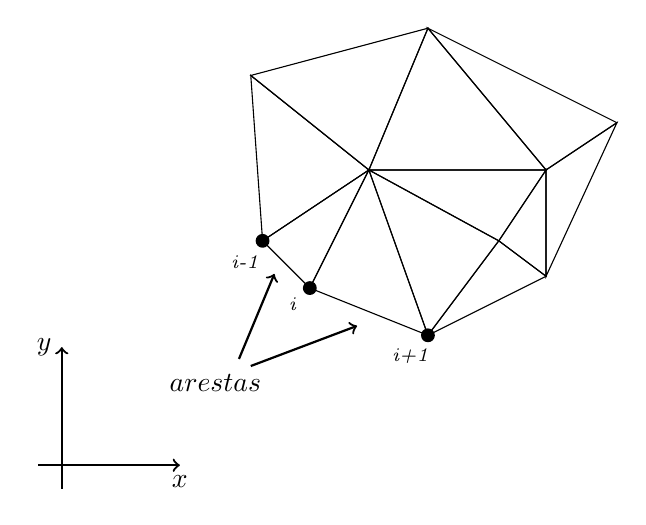
\begin{tikzpicture}[scale=3]
 \draw (0.75,0.75) -- (1.25,0.55) -- (1.00,1.25) -- cycle;
 \draw (0.75,0.75) -- (0.55,0.95) -- (1.00,1.25) -- cycle;
 \draw (1.25,0.55) -- (1.55,0.95) -- (1.00,1.25) -- cycle;
 \draw (1.55,0.95) -- (1.75,1.25) -- (1.00,1.25) -- cycle;
 \draw (1.75,1.25) -- (2.05,1.45) -- (1.25,1.85) -- cycle;
 \draw (1.25,1.85) -- (1.00,1.25) -- (1.75,1.25) -- cycle;
 \draw (1.25,0.55) -- (1.55,0.95) -- (1.75,0.80) -- cycle;
 \draw (1.55,0.95) -- (1.75,0.80) -- (1.75,1.25) -- cycle;
 \draw (1.75,0.80) -- (1.75,1.25) -- (2.05,1.45) -- cycle;
 \draw (0.55,0.95) -- (1.00,1.25) -- (0.50,1.65) -- cycle;
 \draw (1.00,1.25) -- (0.50,1.65) -- (1.25,1.85) -- cycle;
 \node[circle,fill=black, inner sep=0pt, minimum size=5pt] at (0.75,0.75) {};
 \node[circle,fill=black, inner sep=0pt, minimum size=5pt] at (0.55,0.95) {};
 \node[circle,fill=black, inner sep=0pt, minimum size=5pt] at (1.25,0.55) {};
 \node at (0.68,0.68) {\scriptsize \textit{i}};
 \node at (0.48,0.86) {\scriptsize \textit{i-1}};
 \node at (1.18,0.46) {\scriptsize \textit{i+1}};
 \draw [->,thick] (0.45,0.45)--(0.60,0.81);
 \draw [->,thick] (0.50,0.42)--(0.95,0.59);
 \draw [->,thick] (-0.3,-0.1)--(-0.3,0.5) node[left] {$y$};
 \draw [->,thick] (-0.4,0)--(0.2,0) node[below] {$x$};
 \node [draw=none] at (0.35,0.35) {$arestas$};
\end{tikzpicture}
\end{center}
\caption{Arestas vizinhas de um nó}
\end{figure}

\newpage
\noindent
onde a aresta à esquerda do nó \textit{$i$} é constituída
pelos nós \textit{$i-1$} e \textit{$i$}, enquanto a 
aresta à direita é constituída pelos nós \textit{$i$} e \textit{$i+1$}. 
Desta maneira podemos observar que o nó \textit{$i$} recebe
contribuição das aresta a sua esquerda e a sua direita. 
O \textit{script} a seguir é usado para a implementação
da condição de contorno de Neumann quando requerida:


\begin{verbatim}
__________________________________________________________________________
 for i in range(0, len(neumann_edges)):   | loop sobre as arestas neumann
 
  p1 = neumann_edges[i][1]                | os nós que constituem
  p2 = neumann_edges[i][2]                | uma aresta

  x = x[p1] - x[p2]                       | calculo do comprimento
  y = y[p1] - y[p2]                       | de uma aresta
  length = numpy.sqrt(x**2 + y**2)        | 

  bc_neumann[p1] += (length*nabla_c) / 2. | imputando o valor da condição
  bc_neumann[p2] += (length*nabla_c) / 2. | de Neumann no índice
                                          | correspondente.
__________________________________________________________________________

\end{verbatim}

\noindent
onde \textit{neumann\_edges} é uma lista que contém os nós presentes em
uma aresta cuja condição é de Neumann, \textit{p1} e \textit{p2} são os nós 
presentes na aresta, \textit{x} e \textit{y} são as coordenadas de cada nó,
\textit{length} é o comprimento da aresta, \textit{nabla\_c} é o fluxo
adimensional modelado no problema físico e \textit{numpy} é uma biblioteca
numérica do \textit{Python} no qual estamos usando a função da raiz
quadrada (\textit{numpy.sqrt}).
O símbolo += garante que a contribuição das aresta à esquerda e
à direita seja computada.
               
